\documentclass[11pt,letterpaper]{article}

\usepackage[margin=1in]{geometry}
\usepackage[T1]{fontenc}
\usepackage{amsmath}
\usepackage{txfonts}  % Times text and math (with the AMS symbols), close to the STIX fonts in the figures
\usepackage{graphicx}
\usepackage{booktabs}
\usepackage{array}
\usepackage[font=small,labelfont=bf]{caption}
\usepackage[numbers,sort&compress]{natbib}
\usepackage{microtype}
\usepackage{xcolor}
\usepackage[colorlinks=true,linkcolor=blue!50!black,citecolor=blue!50!black,urlcolor=blue!50!black]{hyperref}
\usepackage[capitalise,nameinlink]{cleveref}

\graphicspath{{../figures/}}
\setlength{\parskip}{0.35em}
% Let large figures sit near their text (the defaults push them all to the end)
\renewcommand{\topfraction}{0.9}
\renewcommand{\bottomfraction}{0.8}
\renewcommand{\textfraction}{0.07}
\renewcommand{\floatpagefraction}{0.75}
\setcounter{topnumber}{2}
\setcounter{totalnumber}{4}
\renewcommand{\arraystretch}{1.15}

\newcommand{\avg}[1]{\langle #1 \rangle}
\newcommand{\dd}{\mathrm{d}}
\newcommand{\ee}{\mathrm{e}}

\title{Dynamical Localization in the Quantum Kicked Rotor}
\author{Wei Chen\\[0.3em]\small PHY-315 Quantum Mechanics, final project}
\date{November 2026}

\begin{document}

\maketitle

\begin{abstract}
\noindent
A rotor kicked once per period is the simplest system in which quantum mechanics changes chaotic motion
qualitatively. For strong kicks the classical momentum performs a random walk and the energy grows without
bound. The quantum rotor follows this growth only up to a break time and then stops: its momentum
distribution freezes into an exponentially localized profile, an effect called dynamical localization. We
simulate both versions, the classical one with the Chirikov standard map and the quantum one with an exact
evolution based on the fast Fourier transform, and we check the code against exact results: conservation of
the norm, quantum resonance and antiresonance, the first two kicks, convergence in the number of momentum
states, and time reversal. We then measure the classical diffusion rate $D(K)$ and its Bessel-function
corrections, show the quantum saturation, fit the localization length $\xi$ of the time-averaged momentum
distribution, and test the prediction $\xi \approx D/\hbar^2$ for $\hbar$ from 0.2 to 1 and for kick strengths
$K$ from 4.5 to 11. We find $\xi\hbar^2/D \approx 1.2$ with a scatter of about 20\%, consistent with earlier
work, and $\xi$ follows the oscillations of the classical $D(K)$. Floquet theory and the mapping onto
Anderson localization explain why the growth stops.
\end{abstract}

\tableofcontents

\section{Introduction}
\label{sec:intro}

What does quantum mechanics do to a system whose classical motion is chaotic? Chaos in classical mechanics
means exponential sensitivity to initial conditions: two nearby trajectories separate like $\ee^{\lambda t}$,
where $\lambda$ is the Lyapunov exponent. Quantum mechanics has no trajectories, and the Schr\"odinger equation
is linear, so nothing can separate exponentially in that sense. Yet the classical limit must come out right.
The kicked rotor is the simplest system in which this tension can be studied in full detail, and it is the
subject of this project.

The kicked rotor is a particle on a ring (a rigid rotor) that receives a sharp kick once per period, with a
strength that depends on its angle $\theta$:
\begin{equation}
  H = \frac{p^2}{2} + K\cos\theta\,\sum_{n=-\infty}^{\infty}\delta(t - n).
  \label{eq:hamiltonian}
\end{equation}
Between kicks the rotor turns freely. Integrating Hamilton's equations over one period gives the Chirikov
standard map \cite{Chirikov1979}, one of the most studied models of Hamiltonian chaos. For weak kicks most
orbits are regular and the momentum stays bounded. Above a critical kick strength
$K_c \approx 0.9716$ \cite{Greene1979} the last barrier across the momentum direction breaks, and for
$K \gtrsim 5$ almost all orbits are chaotic. The momentum then performs a random walk: averaged over an
ensemble, $\avg{p^2}$ grows linearly in time, $\avg{p^2} \approx Dn$ after $n$ kicks, with a diffusion rate
$D \approx K^2/2$ plus corrections that oscillate with $K$ \cite{Chirikov1979,Rechester1980,Rechester1981}.

The quantum rotor behaves very differently. Casati, Chirikov, Izraelev and Ford \cite{Casati1979} solved it
numerically in 1979. At first the quantum energy grew like the classical one, but after a break time the
growth slowed down. Later work showed that it stops altogether: the momentum distribution freezes into an
exponentially localized profile $|\psi_m|^2 \sim \ee^{-2|m|/\xi}$ around its starting point. This is
\emph{dynamical localization}. Fishman, Grempel and Prange \cite{Fishman1982} explained it by mapping the
eigenvalue problem of the kicked rotor onto a one-dimensional lattice with pseudo-random on-site energies,
the Anderson model, in which every eigenstate is exponentially localized. The localization length is set by
the classical diffusion rate, $\xi \approx D/\hbar^2$ in our units \cite{Shepelyansky1986,Izrailev1990}. The
effect was observed directly in 1995 with ultracold sodium atoms in a pulsed standing wave of light
\cite{Moore1995}.

In this project we simulate both the classical and the quantum rotor, check the code against exact results,
and then use it to study chaos, diffusion and dynamical localization. The main result is
\cref{fig:quantum_vs_classical}: the quantum energy follows the classical diffusive growth for a few kicks
and then saturates, at a level and after a time that both scale with $\xi$.

The report is organized as follows. \Cref{sec:model} sets up the model, the quantum one-period
(Floquet) operator and the numerical method, and summarizes the validation. \Cref{sec:classical} covers the
classical dynamics: the transition to chaos and the diffusion rate with its Bessel-function corrections.
\Cref{sec:quantum} is the core: Floquet theory, quantum resonance, the break time, the localized momentum
distribution and its localization length, how $\xi$ scales with $K$ and $\hbar$, and the Anderson
analogy. \Cref{sec:correspondence} discusses quantum-classical correspondence and time reversal, and
\cref{sec:experiments} the cold-atom experiment. The appendices contain the derivations of the classical
correlations and of the exact two-kick results, details of the validation tests, and instructions for
reproducing every figure.

\section{Model and method}
\label{sec:model}

\subsection{The classical kicked rotor and the standard map}

We use scaled units in which the kick period and the moment of inertia are both 1, so the Hamiltonian is
\cref{eq:hamiltonian}. Hamilton's equations are $\dot\theta = p$ and
$\dot p = K\sin\theta\,\sum_n\delta(t-n)$. Between kicks the momentum is constant and the angle grows
linearly. Across a kick the angle is continuous and the momentum jumps by $K\sin\theta$. Writing
$(\theta_n, p_n)$ for the state just before kick $n$, one period is
\begin{equation}
  p_{n+1} = p_n + K\sin\theta_n, \qquad \theta_{n+1} = \theta_n + p_{n+1} \pmod{2\pi}.
  \label{eq:standard_map}
\end{equation}
This is the Chirikov standard map \cite{Chirikov1979}. Its Jacobian determinant is 1, so it preserves
phase-space area, as any Hamiltonian flow must. Solving for the earlier state gives the inverse map,
$\theta_n = \theta_{n+1} - p_{n+1}$ and $p_n = p_{n+1} - K\sin\theta_n$, which we use for the time-reversal
test.

The map is unchanged by $p \to p + 2\pi$, so phase space can be drawn on a torus,
$\theta, p \in [0, 2\pi)$, and we do that for the phase portraits. In the dynamics, however, the momentum is
never wrapped, because its unbounded growth is exactly what we want to measure. Small displacements obey the
linearized map $\delta p' = \delta p + K\cos\theta\,\delta\theta$, $\delta\theta' = \delta\theta + \delta p'$.
Their average logarithmic growth rate per kick is the Lyapunov exponent $\lambda$, which we compute by
renormalizing the displacement after every kick.

\subsection{Quantization and the Floquet operator}

Because $\theta$ is an angle, the wave function is periodic, and $\hat p = -i\hbar\,\partial_\theta$ has
eigenvalues $p = \hbar m$ with integer $m$ and eigenfunctions $\ee^{im\theta}/\sqrt{2\pi}$. Here $\hbar$ is the
\emph{effective} Planck constant: in scaled units it is the ratio of Planck's constant to the rotor's action
scale, so it measures how quantum the motion is, and $\hbar\to 0$ is the classical limit.

Integrating the Schr\"odinger equation $i\hbar\,\partial_t\psi = H\psi$ across a kick, the
$\delta$-function term dominates and the kinetic term contributes nothing, so the kick multiplies the wave
function by a phase, $\psi(\theta) \to \ee^{-iK\cos\theta/\hbar}\,\psi(\theta)$, exactly. Between kicks the
rotor is free and each momentum component picks up the phase $\ee^{-i\hbar m^2/2}$. The evolution from just
before one kick to just before the next is therefore given by the one-period (Floquet) operator
\begin{equation}
  \hat U = \ee^{-i\hat p^2/2\hbar}\,\ee^{-iK\cos\hat\theta/\hbar}.
  \label{eq:floquet}
\end{equation}
Its matrix elements in the momentum basis follow from the Jacobi-Anger expansion of the kick,
\begin{equation}
  \ee^{-ik\cos\theta} = \sum_r (-i)^r J_r(k)\,\ee^{ir\theta}
  \quad\Longrightarrow\quad
  \langle m'|\hat U|m\rangle = \ee^{-i\hbar m'^2/2}\,(-i)^{m'-m}\,J_{m'-m}(K/\hbar).
  \label{eq:matrix_elements}
\end{equation}
Because $J_r(k)$ is tiny for $|r| > k$, one kick couples each momentum state to about $k = K/\hbar$
neighbors on either side. So the quantum dynamics depends on two numbers: $K$, which sets the classical
chaos, and $\hbar$, which sets the free phase and, through $k = K/\hbar$, the number of momentum states one
kick connects.

Expectation values in momentum space are sums, for example $\avg{p^2} = \hbar^2\sum_m m^2|\psi_m|^2$. To
compare the two theories we start them in matching states: the quantum rotor in the momentum eigenstate
$m = 0$, which is spread uniformly in angle with zero momentum, and the classical ensemble with $p_0 = 0$ and
$\theta_0$ uniform on $[0, 2\pi)$. After one kick both give exactly $\avg{p^2} = K^2/2$.

\subsection{Numerical method}

We store $\psi$ at $N$ equally spaced angles $\theta_j = 2\pi j/N$. A discrete Fourier transform, computed
with the fast Fourier transform (FFT) and normalized to be unitary, gives the momentum amplitudes $\psi_m$ for
$m = -N/2, \dots, N/2 - 1$. One period is then four steps:
multiply $\psi(\theta_j)$ by $\ee^{-iK\cos\theta_j/\hbar}$, transform to momentum space, multiply $\psi_m$ by
$\ee^{-i\hbar m^2/2}$, and transform back. The inverse step undoes these in reverse order with the conjugate
phases.

This looks like the split-step Fourier method, but it is exact here, with no time-step error. The kick is
diagonal in $\theta$, the free evolution is diagonal in $m$, and the two act at different times rather than
simultaneously, so there is nothing to split. The only approximations are the finite momentum range and
roundoff. The FFT treats momentum as periodic, so probability that reached $|m| = N/2$ would reappear on
the other side. We therefore track the \emph{edge probability}
\begin{equation}
  P_{\rm edge} = \sum_{|m| > 3N/8} |\psi_m|^2
  \label{eq:edge}
\end{equation}
throughout every run and require its largest value to stay below $10^{-10}$. Unless stated otherwise we use
$N = 2^{14} = 16384$ states, chosen by validation check 4 below. One kick then takes about a millisecond on a
laptop.

For the classical ensemble matched to the quantum state we place $M$ angles on the midpoint grid
$\theta_j = 2\pi(j + \tfrac12)/M$ with $p = 0$. Averaging over this grid is the trapezoid rule, which is
extremely accurate for smooth periodic functions, so early-time averages converge much faster than with random
sampling. To measure the diffusion rate $D(K)$ we also use a \emph{torus ensemble}, with $\theta$ and $p$ both
uniform at random (fixed seed). The uniform measure is invariant under the map, so this ensemble has no
start-up transient.

\subsection{Validation}
\label{sec:validation}

Before any physics run, the code had to pass five checks, written as 39 automated tests. Every tolerance in
them has a stated reason: machine precision, the statistical error of an ensemble, or a known physical
correction. \Cref{tab:validation} summarizes them, and \cref{app:validation} gives the details. As a test of
the tests, we planted six deliberate bugs (a wrong free phase, a wrong ordering of the momentum grid, a wrong
classical update, a wrong inverse map, a broken edge probability, and a kick strength off by 0.1\%). Each made
at least one test fail.

\begin{table}[!htbp]
\centering
\small
\begin{tabular}{@{}>{\raggedright}p{0.17\linewidth}>{\raggedright}p{0.36\linewidth}>{\raggedright\arraybackslash}p{0.39\linewidth}@{}}
\toprule
Check & What is tested & Result \\
\midrule
1. Norm & $\avg{\psi|\psi} = 1$ over 1000 kicks, forward and backward & drifts by about $3\times10^{-16}$ per kick
  ($2.9\times10^{-13}$ after 1000), within the FFT roundoff allowance $n\log_2 N\,\varepsilon$ \\
2. Resonance & $\hbar = 4\pi$: $\avg{p^2} = K^2n^2/2$ and $|\psi_m|^2 = J_m^2(nK/\hbar)$;
  $\hbar = 2\pi$: exact return every two kicks & largest relative error $2.9\times10^{-13}$ over 1000 kicks;
  distribution within $1.7\times10^{-15}$; return within $2.8\times10^{-15}$ \\
3. Early times & exact $\avg{p^2}$ after one and two kicks, quantum and classical; at three kicks the quantum
  value approaches the classical one like $\hbar^2$ & quantum within $10^{-14}$ of the formulas; classical
  within the ensemble's error; observed order in $\hbar$: 1.97 \\
4. Grid & $N = 2^{14}$ against $2^{15}$ at $\hbar = 0.25$, 1000 kicks; edge probability below $10^{-10}$ &
  edge probability $2.6\times10^{-27}$; doubling $N$ changes $\avg{p^2}$ only at roundoff level; $N = 2^{12}$
  fails (edge $3.1\times10^{-8}$) \\
5. Time reversal & $n$ kicks forward, then $n$ back & quantum returns within $2.9\times10^{-13}$ after 1000
  kicks; the classical return fails after about 38 kicks, as predicted by $\ln(1/\varepsilon)/\lambda$ \\
\bottomrule
\end{tabular}
\caption{The five validation checks ($\varepsilon = 2.2\times10^{-16}$ is the machine precision; $K = 5$
throughout). Details and the reason for every tolerance are in \cref{app:validation}.}
\label{tab:validation}
\end{table}

\section{Classical dynamics}
\label{sec:classical}

\subsection{From regular motion to global chaos}

\Cref{fig:phase_portraits} shows phase portraits for four kick strengths (experiment 01). The orbits start
on the four symmetry lines of the map, $\theta = 0$, $\theta = \pi$, $\theta = p/2$ and
$\theta = p/2 + \pi$. The standard map is a product of two involutions (maps that are their own inverse), and
these lines are their fixed sets, so symmetric periodic orbits and the islands around them cross them. Each
orbit is classified by its finite-time Lyapunov exponent over kicks 2000 to 4000: chaotic if $\lambda > 0.01$.
On a regular orbit displacements grow only linearly, which gives $\lambda \approx \ln 2/2000$, far below the
threshold.

\begin{figure}[!tbp]
  \centering
  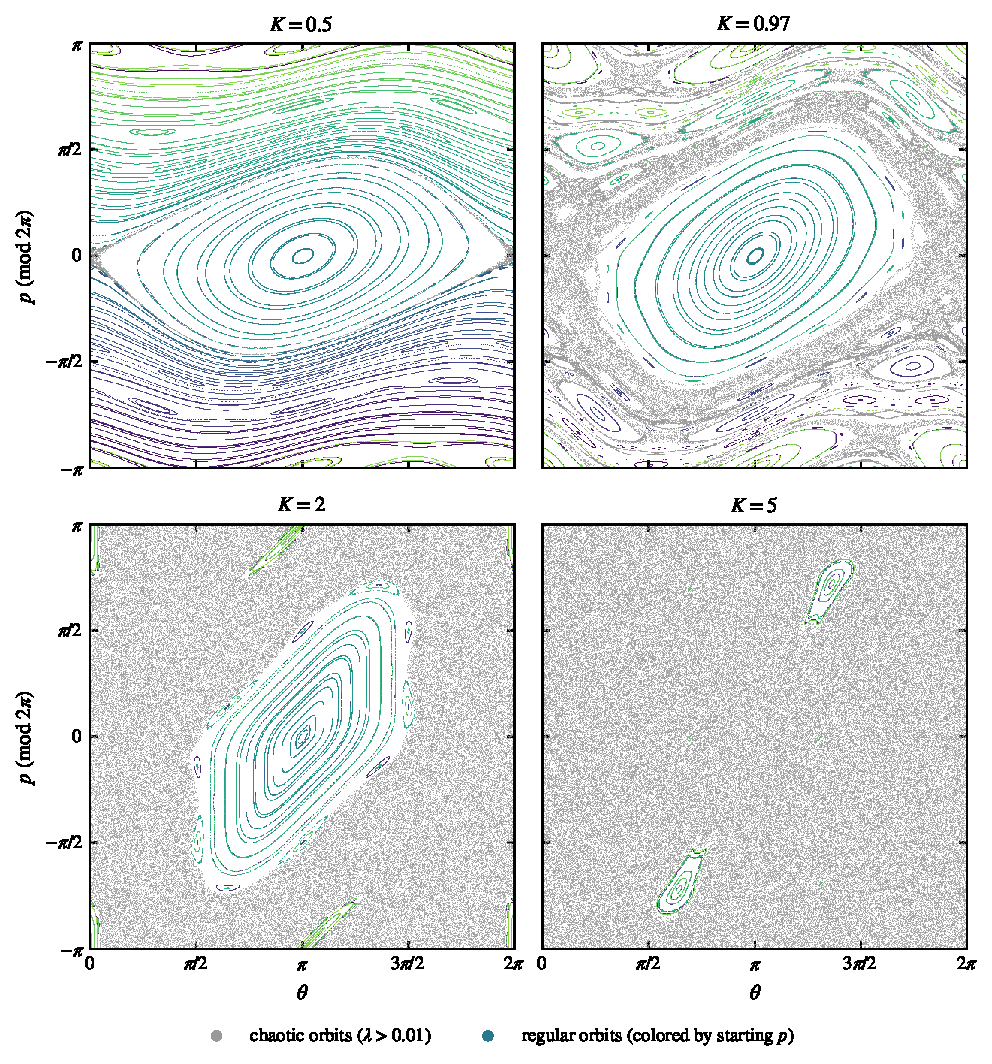
\includegraphics[width=0.78\linewidth]{01_phase_portraits.pdf}
  \caption{Phase portraits of the standard map (experiment 01), with $p$ folded into $[-\pi, \pi)$. Gray:
  chaotic orbits ($\lambda > 0.01$). Colors: regular orbits, colored by their starting momentum. At
  $K = 0.5$ invariant curves span the whole range of $\theta$ and confine the momentum; only a thin chaotic
  layer surrounds the island at $(\pi, 0)$. At $K = 0.97$, just below $K_c = 0.9716$, chaotic layers have
  grown but curves spanning $\theta$ still survive. At $K = 2$ a chaotic sea surrounds the central island,
  and at $K = 5$ almost the whole torus is chaotic, apart from two small islands around a period-2 orbit.}
  \label{fig:phase_portraits}
\end{figure}

\begin{table}[!htbp]
\centering
\small
\begin{tabular}{@{}cccc@{}}
\toprule
$K$ & chaotic area & median $\lambda$ of chaotic orbits & largest $|p_n - p_0|$ in the portrait \\
\midrule
0.5  & 1.2\%  & 0.08 & 2.7 \\
0.97 & 42.6\% & 0.09 & 4.6 \\
2    & 75.5\% & 0.46 & 104 \\
5    & 98.1\% & 0.98 & 628 \\
\bottomrule
\end{tabular}
\caption{Measures of chaos from experiment 01. The chaotic area is the fraction of an $80\times80$ grid of
starting points with $\lambda > 0.01$.}
\label{tab:chaos}
\end{table}

\Cref{tab:chaos} puts numbers on the picture. For weak kicks most orbits are regular, as the
Kolmogorov-Arnold-Moser (KAM) theorem predicts for small perturbations of an integrable system. The
invariant curves that run all the way around in $\theta$ act as walls in momentum: for $K = 0.5$ and 0.97 no
orbit's momentum changes by more than $2\pi$. The last of these curves breaks at
$K_c = 0.971635$, a value Greene found from the stability of periodic orbits that approximate it
\cite{Greene1979}. Above $K_c$ the chaotic layers connect, and a chaotic orbit can wander arbitrarily far in
momentum: at $K = 2$ and 5 the largest momentum changes are 104 and 628 after a few thousand kicks.

Chirikov's resonance-overlap criterion gives a simple estimate of this transition \cite{Chirikov1979}. The
map has resonances at $p = 2\pi n$ with half-width $2\sqrt K$; they overlap when $4\sqrt K \ge 2\pi$, that is,
for $K \ge \pi^2/4 \approx 2.47$. This overestimates the true border by a factor of about 2.5, because
smaller secondary resonances also overlap and destroy the curves earlier, but it captures the mechanism.

The fixed point at $(\theta, p) = (\pi, 0)$ is elliptic for $K < 4$ (its linearized map has trace $2 - K$),
which is why the large central island persists up to $K = 2$. At $K = 5$ it has become unstable, and only
small islands remain, occupying 1.9\% of the torus. For large $K$ the Lyapunov exponent is close to
Chirikov's estimate $\ln(K/2)$ \cite{Chirikov1979}, which comes from averaging $\ln|K\cos\theta|$ over the
chaotic orbit; at $K = 5$ we find $\lambda = 0.98$ against $\ln 2.5 = 0.92$. Chirikov's Table 5.1 lists the
Kolmogorov-Sinai entropy, which for this map equals the mean Lyapunov exponent of the chaotic orbits, divided by
$\ln(K/2)$: 1.20 at $K = 4$ and 1.027 at $K = 6.21$. Our ratio, $0.98/0.92 = 1.07$ at $K = 5$, lies in
between.

\subsection{Diffusion and its Bessel-function corrections}
\label{sec:diffusion}

In the chaotic regime the momentum after $n$ kicks is $p_n = p_0 + K\sum_{j=0}^{n-1}\sin\theta_j$. If the
angles were independent and uniformly distributed, each kick would add $K^2/2$ to the mean square momentum
change, and the motion would be a random walk with the quasilinear diffusion rate
\begin{equation}
  D = \lim_{n\to\infty}\frac{\avg{(p_n - p_0)^2}}{n} = \frac{K^2}{2}.
\end{equation}
Correlations between successive angles change this. With $C_j = \avg{\sin\theta_0\sin\theta_j}$ averaged
over the invariant measure, the exact statement is
\begin{equation}
  D = K^2\Bigl[C_0 + 2\sum_{j\ge1} C_j\Bigr],
  \qquad C_0 = \tfrac12,\quad C_1 = 0,\quad C_2 = -\tfrac12 J_2(K),\quad C_3 = \tfrac12\bigl[J_3^2(K) - J_1^2(K)\bigr],
  \label{eq:D_correlations}
\end{equation}
as derived in \cref{app:correlations}. Keeping lags up to 3 gives the result of Rechester and White
\cite{Rechester1980}, and the first five terms of the later expansion by Rechester, Rosenbluth and White
\cite{Rechester1981} add the leading part of lag 4:
\begin{equation}
  \frac{D}{K^2/2} \approx 1 - 2J_2(K) - 2J_1^2(K) + 2J_3^2(K) + 2J_2^2(K).
  \label{eq:five_term}
\end{equation}
(We have converted their diffusion coefficient, defined with an extra factor $\tfrac12$, to ours.) Since
$J_n(K) \sim \sqrt{2/\pi K}\,\cos(K - n\pi/2 - \pi/4)$ for large $K$, the corrections oscillate with period
$2\pi$ in $K$ and decay like $K^{-1/2}$.

There is one more ingredient. If $K\sin\theta^* = 2\pi l$ for an integer $l$, the point $(\theta^*, p)$
returns to the same angle with its momentum raised by exactly $2\pi l$, so it is a fixed point on the torus
that accelerates forever. It is stable when $|2 + K\cos\theta^*| < 2$, which happens in the windows
$2\pi l \le K \le \sqrt{(2\pi l)^2 + 16}$ \cite{Chirikov1979}, for example $6.28 \le K \le 7.45$ for $l = 1$.
Inside these windows the islands around these \emph{accelerator modes} carry orbits ballistically, and near
them chaotic orbits stick to the islands for long stretches and make long flights. Both effects ruin normal
diffusion, so we keep $K$ away from the windows.

\begin{figure}[!tbp]
  \centering
  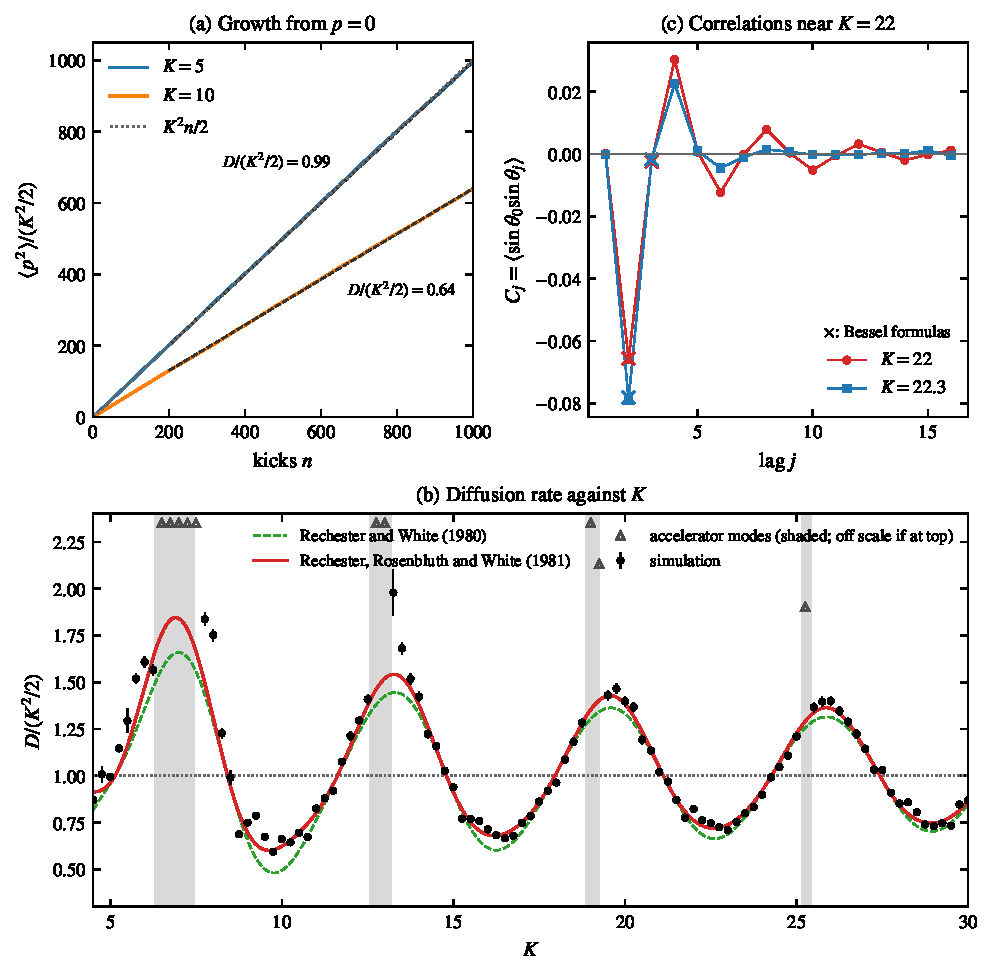
\includegraphics[width=\linewidth]{02_classical_diffusion.pdf}
  \caption{Classical diffusion (experiment 02). (a) $\avg{p^2}/(K^2/2)$ for the ensemble $p_0 = 0$,
  $\theta_0$ uniform (40000 orbits), with the fitted slopes. (b) $D/(K^2/2)$ against $K$ from the torus
  ensemble (10000 orbits per $K$, error bars one standard error), with the four-term formula of
  Rechester and White (dashed), the five-term formula \cref{eq:five_term} (solid), and the accelerator-mode
  windows (shaded; triangles mark values off the scale). (c) The correlations $C_j$ at $K = 22$ and 22.3;
  crosses mark the Bessel-function results for $C_2$ and $C_3$.}
  \label{fig:diffusion}
\end{figure}

\Cref{fig:diffusion} shows the results of experiment 02. Panel (a) confirms linear growth for the
project's ensemble. The slopes give $D/(K^2/2) = 0.995 \pm 0.009$ at $K = 5$ and $0.638 \pm 0.006$ at
$K = 10$, against 0.963 and 0.623 from \cref{eq:five_term}. Panel (b) scans 103 values of $K$ between 4.5 and
30. The measured rate oscillates around the quasilinear value with period about $2\pi$, and away from the
accelerator windows the five-term formula follows it with an rms miss of 0.041. Just outside the windows
the diffusion is strongly enhanced, up to $D/(K^2/2) = 3.2$ at $K = 7.5$.

A few misses are larger than the statistical error allows. In five runs with different random seeds,
$K = 8.75$, 9.25 and 10.75 missed by more than four standard errors every time (by about $-0.11$, $+0.16$
and $-0.06$), and a few other values sat close to that line. Panel (c) shows where such misses come from at
$K = 22$. The measured $C_2 = -0.0658$ and $C_3 = -0.0024$ agree with the Bessel results $-0.0657$ and
$-0.0025$, and the sum up to lag 3 gives 0.728, against 0.727 from the four-term formula. But
$C_4 = +0.030$ adds 0.12 to
$D/(K^2/2)$, and a slowly decaying tail follows, with a sign pattern that repeats every four lags. Summing
the measured correlations up to lag 16 gives 0.823, matching the directly measured 0.821, while the
five-term formula, which contains only the $J_2^2$ part of lag 4, gives 0.762. The truncated formulas are
asymptotic expansions, and they fail wherever the higher correlations happen to be large.

Islands matter for a second reason: they make $D$ depend on the ensemble. At $K = 9.25$ the line $p = 0$
crosses an island that traps about 9\% of the matched ensemble forever. That ensemble gives
$D/(K^2/2) = 0.718$, while the torus ensemble, of which only 0.9\% is trapped, gives 0.800. Both values
are steady over 4000 kicks, so this is not slow convergence. At $K = 4.5$, 5 and every value we tested from
8.75 to 11.25 apart from 9.25, the two ensembles agree to within about two standard errors.

\section{Quantum dynamics}
\label{sec:quantum}

\subsection{Floquet states and quasienergies}
\label{sec:floquet}

Because the Hamiltonian is periodic in time, the evolution over $n$ periods is just $\hat U^n$. The Floquet
operator is unitary, so its eigenvalues lie on the unit circle:
\begin{equation}
  \hat U|\phi_k\rangle = \ee^{-i\omega_k}|\phi_k\rangle, \qquad \omega_k \in [0, 2\pi).
\end{equation}
The phases $\omega_k$ are called quasienergies, and the $|\phi_k\rangle$ Floquet states. They play the role
that energy eigenstates play for a time-independent Hamiltonian. Expanding the initial state as
$|\psi_0\rangle = \sum_k c_k|\phi_k\rangle$ gives
\begin{equation}
  |\psi_n\rangle = \sum_k c_k\,\ee^{-in\omega_k}|\phi_k\rangle,
  \qquad
  \avg{p^2}_n = \sum_{k,k'} c_k^* c_{k'}\,\ee^{in(\omega_k - \omega_{k'})}\,\langle\phi_k|\hat p^2|\phi_{k'}\rangle.
  \label{eq:floquet_expansion}
\end{equation}
Whether the energy can grow without bound depends on the Floquet states. Suppose they are localized in
momentum, $|\phi_k(m)| \sim \ee^{-|m - m_k|/l}$ around some center $m_k$. Then a state started at $m = 0$
overlaps appreciably only with the Floquet states centered within a few $l$ of the origin, so in effect the
sum in \cref{eq:floquet_expansion} has finitely many terms. The energy is then a quasi-periodic function of
$n$: it fluctuates, but it is bounded. Its time average keeps only the diagonal terms (if no two quasienergies
coincide),
\begin{equation}
  \overline{\avg{p^2}} = \sum_k |c_k|^2\,\langle\phi_k|\hat p^2|\phi_k\rangle,
  \qquad
  \overline{P}(m) = \sum_k |c_k|^2\,|\phi_k(m)|^2,
  \label{eq:time_average}
\end{equation}
where $\overline{P}(m)$ is the time-averaged momentum distribution. If instead the spectrum has a
continuous part, with Floquet states extended in momentum, the energy can grow forever. So the question
``does the quantum energy keep growing?'' becomes ``are the Floquet states localized?'' The two exactly
solvable cases below show both possibilities, and the Anderson mapping in \cref{sec:anderson} explains why
localization is the generic answer.

\subsection{Quantum resonance and antiresonance}
\label{sec:resonance}

For special values of $\hbar$ the free phase $\ee^{-i\hbar m^2/2}$ simplifies. At $\hbar = 4\pi$ it equals
$\ee^{-2\pi i m^2} = 1$ for every $m$: the free evolution does nothing, and all kicks add up coherently.
After $n$ kicks the wave function is $\ee^{-inK\cos\theta/\hbar}$, so by the Jacobi-Anger expansion
\begin{equation}
  |\psi_m|^2 = J_m^2(nK/\hbar), \qquad
  \avg{p^2}_n = \hbar^2\sum_m m^2 J_m^2(nK/\hbar) = \frac{K^2 n^2}{2}.
  \label{eq:resonance}
\end{equation}
The energy grows quadratically: the motion is ballistic, faster than any diffusion. This \emph{quantum
resonance} was found by Casati et al.\ \cite{Casati1979}, who also saw quadratic growth at several other
rational values of $\hbar/4\pi$. For a rational $\hbar/4\pi = r/q$ the free phases repeat with period $q$ in
$m$, the Floquet states become extended Bloch waves, and the energy grows without bound
\cite{Izrailev1980,Izrailev1990}.

At $\hbar = 2\pi$ the free phase is $\ee^{-i\pi m^2} = (-1)^m$, which shifts the wave function by $\pi$ in
angle. The next kick then sees $\cos(\theta + \pi) = -\cos\theta$ and undoes the previous one, so
$\hat U^2 = 1$: every state returns exactly after two kicks, for any $K$. Casati et al.\ called this case
``anti-resonant'' \cite{Casati1979}. The energy alternates between $K^2/2$ and 0.

\begin{figure}[!tbp]
  \centering
  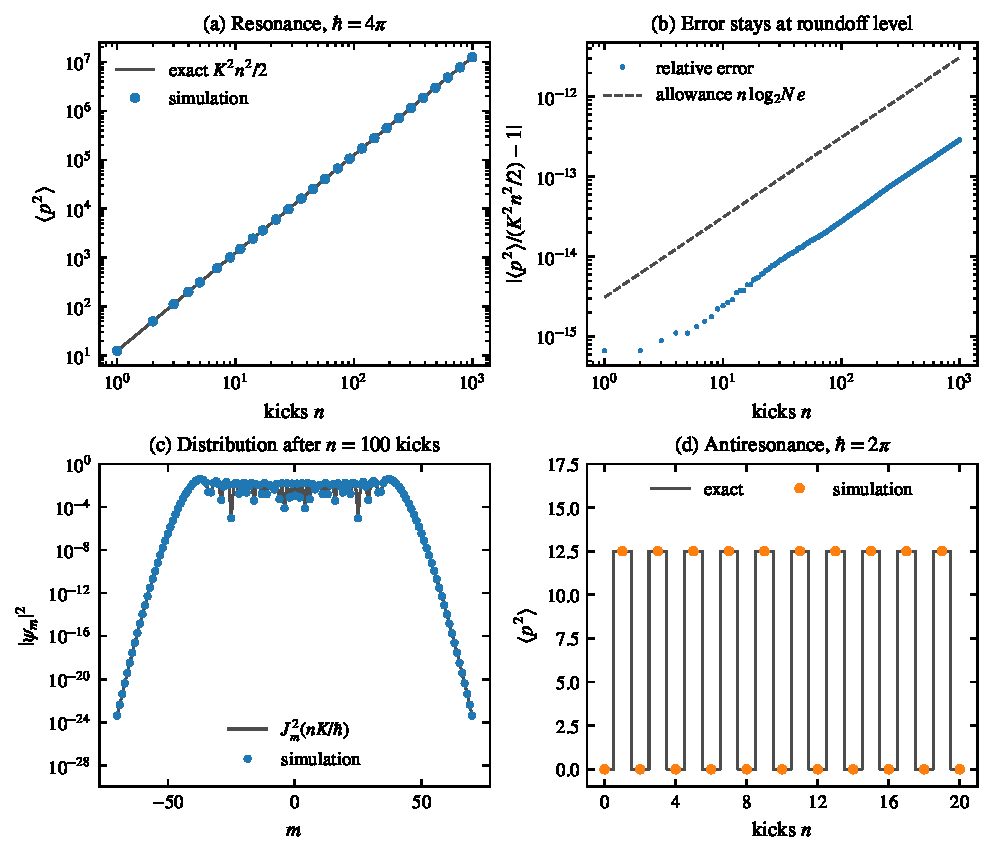
\includegraphics[width=0.85\linewidth]{05_resonance_test.pdf}
  \caption{Quantum resonance and antiresonance at $K = 5$ (experiment 05, validation check 2).
  (a) At $\hbar = 4\pi$ the energy grows as $K^2n^2/2$. (b) The relative error stays below the roundoff
  allowance $n\log_2 N\,\varepsilon$ for $N = 2^{14}$. (c) After 100 kicks the momentum distribution is
  $J_m^2(nK/\hbar)$ over 28 decades. (d) At $\hbar = 2\pi$ the state returns to $m = 0$ after every second
  kick.}
  \label{fig:resonance}
\end{figure}

These exact results make an ideal test of the code (\cref{fig:resonance}). Over 1000 kicks at
$\hbar = 4\pi$ the simulated energy stays within a relative $2.9\times10^{-13}$ of $K^2n^2/2$, an error that
grows linearly with $n$ as roundoff should, and after 100 kicks the distribution matches $J_m^2(nK/\hbar)$
within $1.7\times10^{-15}$. At $\hbar = 2\pi$ the state returns to $m = 0$ within $2.8\times10^{-15}$.

The resonances also tell us what to avoid. In the localization runs, $\hbar/4\pi$ must be irrational and not
too close to a rational with a small denominator. All our standard values ($\hbar = 0.25$, 0.5 and 1) satisfy
this. \Cref{sec:scaling} shows what happens when it fails.

\subsection{Early times: quantum follows classical}
\label{sec:early}

After one kick both theories give exactly $\avg{p^2}_1 = K^2/2$. After two kicks they first differ
(\cref{app:two_kicks}):
\begin{align}
  \avg{p^2}_2^{\rm cl} &= K^2\bigl[1 + J_0(K) - J_2(K) - \tfrac12 J_2(2K)\bigr], \label{eq:two_kicks_cl}\\
  \avg{p^2}_2^{\rm qm} &= K^2\bigl[1 + \cos\tfrac{\hbar}{2}\,\bigl(J_0(K_q) - J_2(K_q)\bigr) - \tfrac12 J_2(K_2)\bigr],
  \qquad K_q = \tfrac{2K}{\hbar}\sin\tfrac{\hbar}{2},\quad K_2 = \tfrac{2K}{\hbar}\sin\hbar. \label{eq:two_kicks_qm}
\end{align}
As $\hbar \to 0$, $K_q \to K$ and $K_2 \to 2K$, and the quantum result goes over into the classical one.
The difference is of order $\hbar^2$: at $K = 5$ the quantum value is lower by 0.18\% at $\hbar = 0.1$ and by
1.0\% at $\hbar = 0.25$. (At $\hbar = 4\pi$ the formula gives $2K^2$, the resonance value, and at
$\hbar = 2\pi$ it gives 0, the antiresonance.) Both formulas are reproduced by the code to machine precision
(check 3).

At later times the agreement deteriorates quickly. Since $\avg{p^2}$ is even in $\hbar$, the quantum value
approaches the classical one as $c + a\hbar^2 + O(\hbar^4)$, but the coefficient $a$ grows rapidly with the
number of kicks: about $-0.2$ at $n = 2$, $-35$ at $n = 3$ and roughly $-550$ at $n = 4$ (relative to the
classical value, $K = 5$). At $\hbar = 0.05$ the three-kick gap is already 6\%. This is the Ehrenfest time at
work: chaotic stretching magnifies quantum effects by about $\ee^{\lambda}$ per kick, so detailed
correspondence lasts only for $t_E \sim \lambda^{-1}\ln(1/\hbar)$, a few kicks here; after that ``only rough
statistical properties like diffusion remain'' \cite{Izrailev1990}. The correspondence limit still holds at
fixed $n$: from $\hbar = 0.02$, 0.01 and 0.005 the gap at $n = 3$ shrinks with an observed order of 1.97 in
$\hbar$, and a Richardson extrapolation recovers the classical $\avg{p^2}_3 = 32.25286$ within
$1.2\times10^{-4}$ (check 3).

\subsection{Dynamical localization}
\label{sec:localization}

Diffusion survives the Ehrenfest time, but not forever. A simple estimate shows when it must stop. Suppose
the Floquet states are localized with a length of order $\xi$ momentum states. Then the initial state
overlaps with roughly $\xi$ of them, and their quasienergies, spread over $[0, 2\pi)$, have a mean spacing of
about $2\pi/\xi$. The evolution cannot resolve this spacing before a time of order $t^* \sim \xi$ kicks (the
analog of the Heisenberg time $\hbar/\Delta E$). Before $t^*$ the dynamics does not know the spectrum is
discrete, and the momentum diffuses as in the classical system, $\avg{m^2} \approx Dn/\hbar^2$; after $t^*$ it
stops. Consistency requires $\xi^2 \sim \avg{m^2}(t^*) \sim Dt^*/\hbar^2 \sim D\xi/\hbar^2$, so
\begin{equation}
  \xi \sim \frac{D}{\hbar^2}, \qquad t^* \sim \frac{D}{\hbar^2}, \qquad
  \avg{p^2}_\infty \sim \hbar^2\xi^2 \sim \frac{D^2}{\hbar^2}.
  \label{eq:estimates}
\end{equation}
The localization length is the classical diffusion rate measured in momentum states per kick. The smaller
$\hbar$, the longer the classical-like growth lasts and the higher the energy at which it saturates, but for
any $\hbar > 0$ the growth eventually stops. The classical limit $\hbar\to0$ and the long-time limit
$n\to\infty$ do not commute.

\begin{figure}[!tbp]
  \centering
  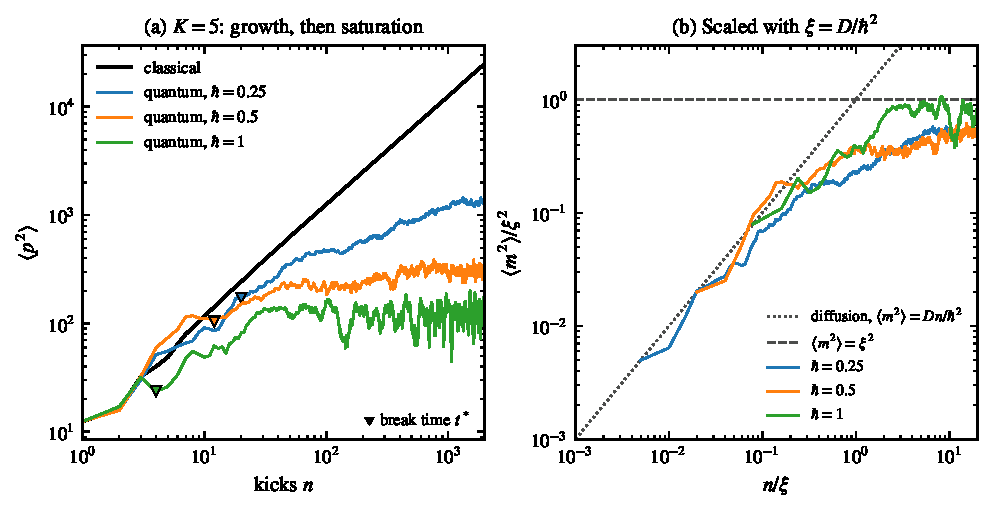
\includegraphics[width=\linewidth]{03_quantum_vs_classical.pdf}
  \caption{The main result (experiment 03, $K = 5$). (a) The classical energy (black, 40000 orbits) grows
  linearly forever. The quantum energy (colors, starting in $m = 0$) follows it at first and then saturates;
  triangles mark the break time $t^*$, after which the quantum energy stays more than 25\% below the classical
  one. (b) The same curves in units of $\xi = D/\hbar^2$: $\avg{m^2}/\xi^2$ against $n/\xi$. The dotted line is
  the diffusive growth $\avg{m^2} = Dn/\hbar^2$, the dashed line $\avg{m^2} = \xi^2$.}
  \label{fig:quantum_vs_classical}
\end{figure}

\Cref{fig:quantum_vs_classical} shows exactly this behavior (experiment 03). The classical ensemble diffuses
with $D = 12.51 \pm 0.10$, that is, $D/(K^2/2) = 1.001$. The quantum curves for $\hbar = 0.25$, 0.5 and 1
follow it and then bend over and saturate. We define the break time as Izrailev does \cite{Izrailev1990}: the
first kick from which the quantum energy stays more than 25\% below the classical one. This gives
$t^* = 20$, 12 and 4 kicks, or 0.10, 0.24 and 0.32 times $\xi = D/\hbar^2$; the estimate $t^* \sim \xi$ is only
an order of magnitude, and with this criterion the break comes earlier. Averaged over kicks 1000 to 2000, the
saturated energies are 1305, 300 and 119, which is 0.52, 0.48 and 0.76 times $D^2/\hbar^2$. For
$\hbar = 0.25$, Izrailev's Fig.~1 shows the same case over 2000 kicks; read off the figure, his energy levels
off near $\avg{p^2} \approx 1400$, consistent with ours.

The saturated energy is not constant. In a run of 40000 kicks at $\hbar = 0.25$, the averages over blocks of
2500 kicks ranged from 1100 to 1960 around a mean of about 1500 (17\% rms), with no upward trend. Such slow
swings are what \cref{eq:floquet_expansion} predicts: the energy is a sum of terms oscillating at the
differences of nearby quasienergies, some of which are very small.

Panel (b) of \cref{fig:quantum_vs_classical} rescales the curves with $\xi = D/\hbar^2$. Diffusion is then
the same line for all three values of $\hbar$, and all three curves leave it near $n/\xi \approx 0.1$ and
level off between 0.5 and 1 times $\xi^2$. The collapse is not perfect, but it confirms that $\xi$ sets both
the break time and the saturation level.

\subsection{The localized momentum distribution}
\label{sec:distribution}

The time-averaged momentum distribution \cref{eq:time_average} is the clearest signature of localization.
If the Floquet states were simple exponentials with a fixed length, $\overline{P}(m)$ would be a sum of
exponentials. Shepelyansky \cite{Shepelyansky1986} found that the Floquet states decay like
$|\phi(m)|^2 \sim \ee^{-2|m|/l}$ with $l \approx D/(2\hbar^2)$, and that the time-averaged distribution of a
state started at $m = 0$ decays about twice as slowly, because the Floquet states fluctuate strongly; from
Chirikov and Shepelyansky's data its length is $l_s = (1.04 \pm 0.20)\,D/\hbar^2$ (mean and rms spread).
Izrailev \cite{Izrailev1990} gives its shape,
\begin{equation}
  \overline{P}(m) = \frac{1}{2\xi}\Bigl(1 + \frac{2|m|}{\xi}\Bigr)\ee^{-2|m|/\xi},
  \qquad \avg{m^2} = \xi^2,
  \label{eq:izrailev_shape}
\end{equation}
with $\xi = l_s \approx D/\hbar^2$. This defines our localization length: $|\psi_m|^2 \sim \ee^{-2|m|/\xi}$
in the tails. (Moore et al.\ \cite{Moore1995} define the localization length as the $1/e$ point of the
probability, which is half of ours.) The prefactor matters for fitting: fitting a pure exponential to
\cref{eq:izrailev_shape} overestimates $\xi$ by 31\% over $\xi/2 \le |m| \le 3\xi$ and still by 7\% over
$4\xi \le |m| \le 10\xi$. So we fit the full shape, in $\ln\overline{P}$, from $|m| = 5$ (past the central
peak) out to where $\overline{P}$ falls to $10^{-14}$ of its maximum.

\begin{figure}[!tbp]
  \centering
  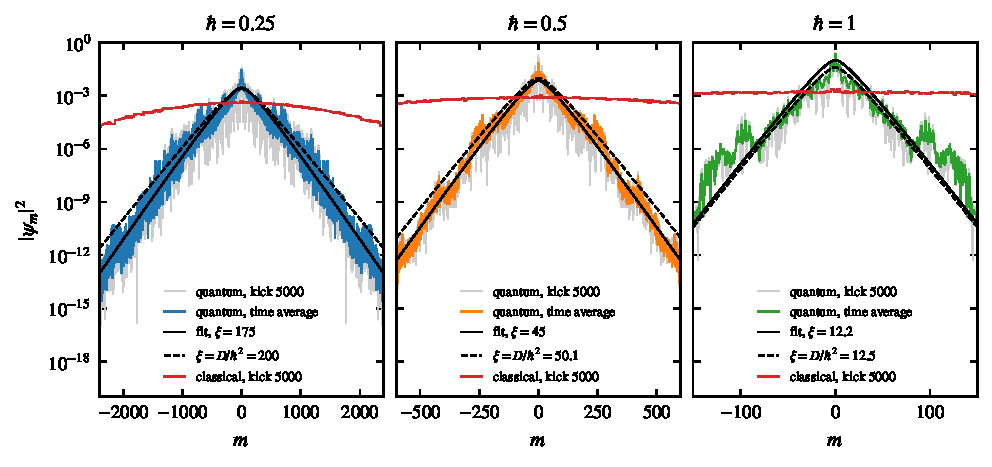
\includegraphics[width=\linewidth]{04_momentum_distribution.pdf}
  \caption{The localized momentum distribution at $K = 5$ (experiment 04). Colors: the quantum distribution
  averaged over kicks 2500 to 5000; gray: the distribution at kick 5000; black solid: the fit of
  \cref{eq:izrailev_shape}; black dashed: the same shape with $\xi = D/\hbar^2$; red: the classical
  distribution at kick 5000 (bins with fewer than 10 of the 40000 orbits are not drawn). Note the 20 decades
  on the vertical axis.}
  \label{fig:distribution}
\end{figure}

\Cref{fig:distribution} shows the result (experiment 04). On a logarithmic scale the quantum distributions
are straight-sided tents: exponential localization, over 13 decades at $\hbar = 0.25$. The classical
distribution at the same time is a broad Gaussian, nearly flat on this scale, with width
$\sqrt{Dn}/\hbar = 1000$ states at $\hbar = 0.25$ and still growing like $\sqrt n$. The fitted localization
lengths are 175, 45.0 and 12.2 states, or 0.87, 0.90 and 0.98 times $D/\hbar^2$, inside the spread of
Shepelyansky's data. Three caveats come with these numbers:
\begin{itemize}
  \item The far tails fill in slowly, so the fit depends on the averaging window. Averaging over kicks 1000 to
  2000 instead gives 0.80, 0.84 and 0.97. A 40000-kick run at $\hbar = 0.25$ levels off at 0.90 to 0.92 for
  windows from 5000 kicks on: the tail at $|m| \approx 3000$ (about $15\xi$) rises from $10^{-17.7}$ in the
  early window to about $10^{-14.6}$ and then stays there.
  \item At $\hbar = 1$ only about a dozen states are involved and the distribution is bumpy: fitting only the
  inner half of the range gives 17 to 18.5 instead of 12.2.
  \item The distributions have a narrow central peak that \cref{eq:izrailev_shape} lacks. The states
  $|m| < 5$ hold 9\% of the probability at $\hbar = 0.25$ and 19\% at $\hbar = 0.5$, against 3\% and 6\% under
  the fitted shape. This is why $\sqrt{\avg{m^2}}$ (154 and 34) comes out below the fitted $\xi$ (175 and 45).
  We have not identified its cause.
\end{itemize}
The distribution at a single kick (gray) fluctuates strongly around the time average. These fluctuations are
the beats between nearby quasienergies in \cref{eq:floquet_expansion}, and they can be large: at
$\hbar = 0.25$ the states near $|m| \approx 680$ hold up to 1.3\% of the probability around kick 1500, more
than twice their time average of 0.6\%, before it drains away again. An animation of the distribution, quantum against classical, is in
\texttt{figures/04\_momentum\_distribution.gif}: the classical Gaussian keeps widening while the quantum
tent stops spreading after a few hundred kicks.

\subsection{How the localization length scales with \texorpdfstring{$\hbar$}{hbar} and \texorpdfstring{$K$}{K}}
\label{sec:scaling}

Experiment 07 tests $\xi \approx D/\hbar^2$ over a wider range (\cref{fig:scaling}). Each run starts in
$m = 0$, lasts at least 5000 kicks and at least $50\,D/\hbar^2$ kicks, and fits \cref{eq:izrailev_shape} to
the time average over its second half. The grid is enlarged until the edge probability stays below
$10^{-10}$ and the fit range lies well inside it. The classical $D$ is measured at each $K$ with the matched
ensemble, and $K$ is kept away from the accelerator windows and from $K = 9.25$ (\cref{sec:diffusion}).

\begin{figure}[!tbp]
  \centering
  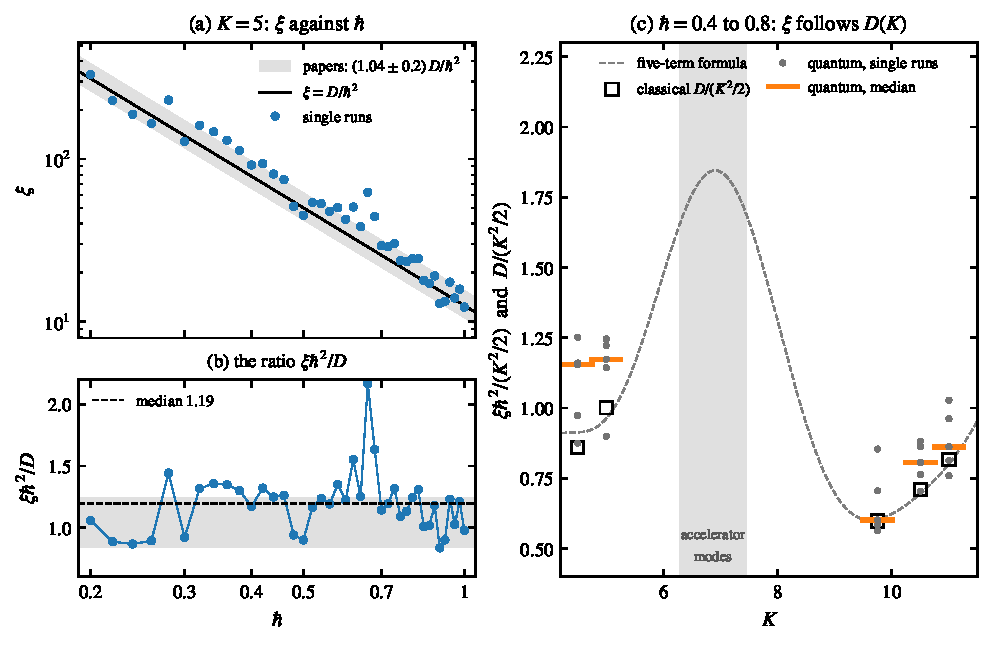
\includegraphics[width=\linewidth]{07_bonus_xi_scaling.pdf}
  \caption{Scaling of the localization length (experiment 07). (a) $\xi$ against $\hbar$ at $K = 5$ for 41
  single runs, with $\xi = D/\hbar^2$ (line) and Shepelyansky's $(1.04\pm0.20)\,D/\hbar^2$ (band). (b) The
  ratio $\xi\hbar^2/D$ for the same runs. (c) $\xi\hbar^2/(K^2/2)$ for five values of $\hbar$ between 0.4 and
  0.8 (dots) and their median (bars), against the measured classical $D/(K^2/2)$ (squares) and the five-term
  formula \cref{eq:five_term} (dashed).}
  \label{fig:scaling}
\end{figure}

Panel (a) shows 41 runs at $K = 5$ with $\hbar$ from 0.20 to 1.00. While $\xi$ falls by a factor of about
27, from 330 to 12, it follows $D/\hbar^2$ closely. Panel (b) shows the ratio $\xi\hbar^2/D$: its median is
1.19 and its rms spread 0.25, compared with $1.04 \pm 0.20$ from Shepelyansky's data. The scatter is not
random from point to point, though. The ratio wanders in broad bands, about 0.89 for $\hbar < 0.3$, about 1.25
from 0.3 to 0.75 and about 1.09 above, and values of $\hbar$ only 0.01 apart give strongly correlated
results (correlation coefficient 0.57 between neighbors in a finer scan). We do not know the cause of these
bands. The known quantum correction to the diffusion rate, replacing $K$ by $K_q$ in the Bessel functions
\cite{Izrailev1990}, changes $D$ by only about 2\% at $\hbar = 0.35$, far too little.

Panel (c) varies the kick strength at fixed $\hbar$. The naive estimate $D = K^2/2$ would make
$\xi\hbar^2/(K^2/2)$ constant. Instead it follows the measured classical $D/(K^2/2)$: about 1.15 at
$K = 4.5$ and 5, then down to 0.60 at $K = 9.75$, exactly where the classical diffusion has its Bessel dip
(0.60), and back up to 0.81 and 0.86 at $K = 10.5$ and 11. The quantum localization length inherits the
oscillations of the classical diffusion rate.

Finally, a warning about resonances. In an earlier version of this experiment, one run at $\hbar = 0.714$
gave $\xi\hbar^2/D = 4.8$ and pushed probability to the edge of a 2048-state grid. The reason is arithmetic:
$0.714/4\pi$ differs from $5/88$ by only $1.4\times10^{-7}$, so the free phases repeat with period 88 out to
$|m| \sim 1000$, and the state spreads as if at a resonance. The final version of the experiment would report such a run as
not localized instead of fitting it; none of the runs in \cref{fig:scaling} needed that.

\subsection{The Anderson localization analogy}
\label{sec:anderson}

Why are the Floquet states localized? Fishman, Grempel and Prange \cite{Fishman1982} answered this by
turning the Floquet eigenvalue problem into a tight-binding model. Write the kick as
\begin{equation}
  \ee^{-ik\cos\theta} = \frac{1 + iW(\theta)}{1 - iW(\theta)}, \qquad W(\theta) = -\tan\Bigl(\frac{k\cos\theta}{2}\Bigr),
  \qquad k = \frac{K}{\hbar},
\end{equation}
and look for a Floquet state $\hat U|u\rangle = \ee^{-i\omega}|u\rangle$ in the form $u = (1 - iW)v$. The free
phases are diagonal in $m$, and a few lines of algebra turn the eigenvalue equation into
\begin{equation}
  T_m v_m + \sum_{r\ne0} W_r\,v_{m+r} = -W_0\,v_m,
  \qquad T_m = \tan\Bigl(\frac{\omega - \hbar m^2/2}{2}\Bigr),
  \label{eq:anderson}
\end{equation}
where $W_r$ are the Fourier coefficients of $W(\theta)$. This is the equation for a particle hopping on a
one-dimensional lattice, whose sites are the momentum states $m$. The hopping amplitudes $W_r$ come from the
kick, and $T_m$ plays the role of an on-site energy.

When $\hbar/4\pi$ is irrational, the phases $\hbar m^2/2 \bmod 2\pi$ are spread uniformly and in an
irregular order, so $T_m$, the tangent of a uniformly distributed angle, behaves like a random number with a
Cauchy (Lorentzian) distribution. \Cref{eq:anderson} is then the Lloyd model, a version of the Anderson model
of a particle in a random potential, in which all eigenstates in one dimension are exponentially localized.
The localized Floquet states in momentum are the analog of localized electron states in a disordered wire,
with the time-periodic kicking playing the role of the disorder. When $\hbar/4\pi$ is rational, $T_m$ is
periodic in $m$, the eigenstates are extended Bloch waves, and the energy grows: the quantum resonance of
\cref{sec:resonance}. The ``disorder'' here is deterministic, though, which is why the arithmetic of
$\hbar/4\pi$ matters, as the near-resonant run of \cref{sec:scaling} showed.

The analogy explains why the Floquet states are localized, but not how long they are. For that we need the
diffusion argument of \cref{sec:localization} and numerical results such as Shepelyansky's
$l \approx D/(2\hbar^2)$ for the Floquet states \cite{Shepelyansky1986} and the measurements of
\cref{sec:distribution,sec:scaling}.

\section{Quantum-classical correspondence and time reversal}
\label{sec:correspondence}

The two theories follow each other closely for a short time and statistically for longer, and then part
ways for good. A time-reversal experiment shows the deeper difference behind this (experiment 06,
\cref{fig:time_reversal}). We run $n$ kicks forward, then $n$ kicks backward with the exact inverse map or the
exact inverse Floquet step, and measure how far the result is from the starting point. Without roundoff both
would return exactly.

\begin{figure}[!tbp]
  \centering
  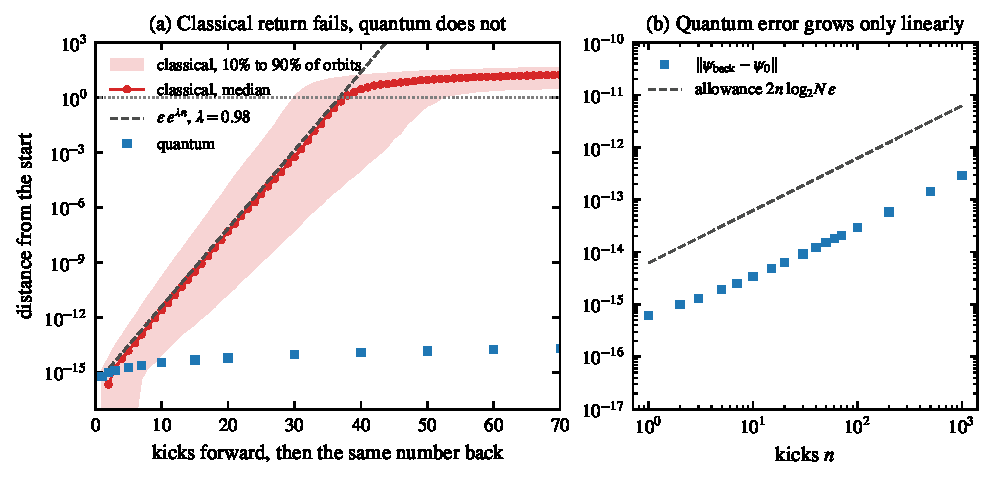
\includegraphics[width=\linewidth]{06_time_reversal.pdf}
  \caption{Time reversal at $K = 5$ (experiment 06). (a) Distance from the starting point after $n$ kicks
  forward and $n$ back. Red: median over 4000 classical orbits ($p_0 = 0$, $\theta_0$ uniform), with the band
  from the 10th to the 90th percentile; dashed: $\varepsilon\,\ee^{\lambda n}$ with the measured
  $\lambda = 0.98$. Blue: the quantum state ($\hbar = 0.25$, $N = 2^{14}$). (b) The quantum error up to 1000
  kicks, against the roundoff allowance $2n\log_2 N\,\varepsilon$.}
  \label{fig:time_reversal}
\end{figure}

For the classical orbits each step rounds the result to about $\varepsilon = 2.2\times10^{-16}$, and chaos
stretches such an error by about $\ee^{\lambda}$ per kick. The median return distance indeed grows like
$1.5\times10^{-16}\,\ee^{0.972n}$, close to the measured $\lambda = 0.981$ of the same orbits, and it first
exceeds 1 at $n = 38$, against the prediction $\ln(1/\varepsilon)/\lambda = 36.7$. After that the
``reversed'' orbits are as far from their starting points as random points on the chaotic sea. The quantum
state, on the other hand, returns to within $3.4\times10^{-15}$ after 10 kicks forward and back,
$3.0\times10^{-14}$ after 100 and $2.9\times10^{-13}$ after 1000. The error grows only linearly, at about a
twentieth of the roundoff allowance.

The reason is that the Schr\"odinger equation is linear and its evolution unitary. If $\delta$ is the error
made at some step, then $\|\hat U(\psi + \delta) - \hat U\psi\| = \|\delta\|$: later steps carry the error
along without magnifying it, and the errors from different steps at most add up. Exponential sensitivity in
the sense of classical chaos is impossible for a wave function. It is worth noting that the classical
Liouville equation for a phase-space density is also linear and conserves the density's norm. What amplifies
roundoff is following individual trajectories, not classical mechanics as such.

We also saw this effect without intending to. The same code run on a Windows laptop and on a Linux server
gave every quantum number to all printed digits, but every classical number came out slightly different: for
example $D = 12.44 \pm 0.10$ on one and $12.51 \pm 0.10$ on the other. The only operation in the standard
map that IEEE floating-point arithmetic does not fix exactly is the sine, which the two NumPy builds can
round differently in the last bit. Chaos amplifies that difference until, after about 37 kicks at $K = 5$,
every orbit is different, and ensemble averages then agree only within their statistical errors (which we
checked: 32 independent ensembles of 40000 orbits scatter by 0.103 around the mean $D$, against a stated
error of 0.099). At $K = 22$, where $\lambda \approx \ln 11 \approx 2.4$, the two machines' correlation sums
of \cref{fig:diffusion}(c) agree through lag 8 and differ by lag 16: roundoff needs only about 15 kicks to
grow to order 1 there.

Putting this together, there are three time scales. Up to the Ehrenfest time
$t_E \sim \lambda^{-1}\ln(1/\hbar)$, a few kicks, quantum expectation values follow the classical ones in
detail. Up to the break time $t^* \sim D/\hbar^2$, they follow them only statistically: the energy grows at
the classical diffusion rate even though individual quantities differ. After $t^*$ the discreteness of the
quasienergy spectrum takes over and the growth stops. For $\hbar = 0.25$, $t_E$ is about one kick, the 25\%
criterion puts the break at 20 kicks, and the saturation is complete after a few hundred kicks, of the order
of $\xi = 200$. The classical limit is recovered as $\hbar\to0$ at fixed $n$, because both $t_E$ and $t^*$ go to
infinity, but at any fixed $\hbar$ the long-time behavior is fundamentally quantum.

\section{Dynamical localization in the laboratory}
\label{sec:experiments}

Moore, Robinson, Bharucha, Sundaram and Raizen realized the quantum kicked rotor with ultracold sodium
atoms in 1995 \cite{Moore1995}. The atoms move in a standing wave of near-resonant laser light, whose
intensity pattern acts on them as a potential proportional to $\cos(2k_L x)$, with $k_L$ the wave number of
the light. Switching the standing wave on in short pulses with period $T$ turns this into a kicked rotor, with
the angle $\theta = 2k_L x$ and the momentum measured in units of $2\hbar k_L$. The kick strength $\kappa$ plays
the role of our $K$, and the scaled Planck constant $\bar k = 8\omega_r T$, where $\omega_r$ is the atomic
recoil frequency, plays the role of our $\hbar$. Because $\bar k$ depends on the pulse period, the experiment
can tune how quantum the motion is.

In their main run ($\kappa = 11.6$ with a 10\% uncertainty, $\bar k = 2.0$) the momentum spread first grew
diffusively at the classical rate $\kappa^2/2$ and then stopped after a break time of about 8 kicks. From then
on the momentum distribution stayed exponentially localized, checked out to 50 kicks. They quote a
localization length $\xi = \kappa^2/4\bar k^2 \approx 8.3$ in units of $2\hbar k_L$, defined as the $1/e$ point
of the probability distribution, $P \propto \ee^{-|n|/\xi}$. In our convention, with $|\psi_m|^2 \propto
\ee^{-2|m|/\xi}$, this is twice as long, $\kappa^2/2\bar k^2 = D/\hbar^2$, exactly the estimate of
\cref{eq:estimates}.

They also observed quantum resonances, when $\bar k/2$ was a rational multiple of $2\pi$. At odd multiples of
$\pi$ (our antiresonance, $\hbar = 2\pi$) the first two or three kicks showed the predicted sign flip, with the
second kick undoing the first. One difference from our idealized model: the atoms start in a Gaussian wave
packet rather than a single momentum state, so at resonance their distributions stayed narrow instead of
growing quadratically. For a review of chaos experiments with cold atoms see Saif \cite{Saif2005}.

Dynamical localization is an interference effect between Floquet states, so it needs phase coherence.
Anything that randomizes the phase of the wave function between kicks, such as the spontaneous emission of a
photon or noise in the kick strength, would break the interference that stops the growth. In this respect too
it resembles Anderson localization of electrons, which inelastic scattering destroys.

\section{Conclusions}
\label{sec:conclusions}

We built a simulation of the classical and quantum kicked rotor, validated it against exact results, and
used it to follow how a quantum system suppresses chaotic diffusion. The main findings are:
\begin{itemize}
  \item For $K$ above $K_c \approx 0.97$ the classical momentum diffuses, with $D/(K^2/2)$ oscillating around 1
  with period about $2\pi$ in $K$. The Bessel-function expansion reproduces this to an rms miss of 0.04, and
  where it misses, the cause is visible in the measured correlations of the kick sequence. Islands, in
  particular the accelerator modes, make the diffusion anomalous or ensemble dependent.
  \item The quantum energy follows the classical growth at first: exactly after one kick, to order $\hbar^2$
  after two, in detail up to the Ehrenfest time, and statistically up to a break time $t^* \sim D/\hbar^2$.
  Then it saturates at about $0.5$ to $0.8$ times $D^2/\hbar^2$ and only fluctuates.
  \item The time-averaged momentum distribution is exponentially localized, with the shape predicted by
  Izrailev. Its localization length is $\xi \approx 1.2\,D/\hbar^2$ with a scatter of about 20\% over
  $0.2 \le \hbar \le 1$, consistent with the $(1.04 \pm 0.20)\,D/\hbar^2$ from earlier work, and it follows the
  oscillations of the classical $D(K)$.
  \item Floquet theory explains why the growth stops (a discrete quasienergy spectrum makes the energy
  quasi-periodic), and the mapping onto the Anderson model explains why the Floquet states are localized.
  At rational $\hbar/4\pi$ the localization fails, and we reproduced the exact resonance and antiresonance.
  \item Quantum evolution does not amplify errors, while classical chaos amplifies them exponentially, as the
  time-reversal experiment and the comparison of two computers both show.
\end{itemize}

Some observations remain unexplained: the broad bands in $\xi\hbar^2/D$ as $\hbar$ varies, the narrow central
peak of the time-averaged distribution, and the long-range correlations behind the misses of the diffusion
formula at a few values of $K$. Each would make a good follow-up. The code is modular, so further numerical
studies, for example of the statistics of the quasienergies or of how noise destroys localization, can build
on it directly.


\appendix
\section{The classical correlations and the Bessel corrections}
\label{app:correlations}

\paragraph{Diffusion from correlations.}
After $n$ kicks, $p_n - p_0 = K\sum_{j=0}^{n-1}\sin\theta_j$. Averaging over the uniform measure on the torus,
which the map preserves, the correlation $\avg{\sin\theta_i\sin\theta_j}$ depends only on $|i - j|$; call it
$C_{|i-j|}$. Then
\begin{equation}
  \avg{(p_n - p_0)^2} = K^2\sum_{i,j=0}^{n-1} C_{|i-j|} = K^2\Bigl[nC_0 + 2\sum_{j=1}^{n-1}(n - j)\,C_j\Bigr],
\end{equation}
and if the $C_j$ decay fast enough, dividing by $n$ and letting $n\to\infty$ gives
$D = K^2\bigl[C_0 + 2\sum_{j\ge1}C_j\bigr]$, which is \cref{eq:D_correlations}.

\paragraph{Angles as independent variables.}
Eliminating the momentum from \cref{eq:standard_map} gives the second-order form
$\theta_{j+1} = 2\theta_j - \theta_{j-1} + K\sin\theta_j$. The change of variables
$(\theta_0, p_0) \mapsto (\theta_0, \theta_1)$ with $\theta_1 = \theta_0 + p_0 + K\sin\theta_0$ is a shear
with unit Jacobian, so if $(\theta_0, p_0)$ is uniform on the torus, so is $(\theta_0, \theta_1)$: the first
two angles are independent and uniform, and all later angles follow from them. Averages of
$\ee^{i(a\theta_0 + b\theta_1)}$ with integers $a, b$ vanish unless $a = b = 0$. Writing
\begin{equation}
  C_j = \tfrac12\,\mathrm{Re}\bigl[\avg{\ee^{i(\theta_0 - \theta_j)}} - \avg{\ee^{i(\theta_0 + \theta_j)}}\bigr]
\end{equation}
and expanding with the Jacobi-Anger identity $\ee^{iz\sin\theta} = \sum_l J_l(z)\,\ee^{il\theta}$, each
correlation reduces to picking out the terms in which all angles cancel.

\paragraph{The first lags.}
$C_0 = \avg{\sin^2\theta_0} = \tfrac12$. Since $\theta_1$ is independent of $\theta_0$, $C_1 = 0$. For lag 2,
\begin{equation}
  \ee^{i\theta_2} = \ee^{-i\theta_0}\,\ee^{2i\theta_1}\,\ee^{iK\sin\theta_1}
  = \ee^{-i\theta_0}\sum_l J_l(K)\,\ee^{i(2+l)\theta_1}.
\end{equation}
In $\avg{\ee^{i(\theta_0 + \theta_2)}}$ the $\theta_0$ dependence cancels and only $l = -2$ survives, giving
$J_{-2}(K) = J_2(K)$; $\avg{\ee^{i(\theta_0 - \theta_2)}}$ contains $\ee^{2i\theta_0}$ and vanishes. So
$C_2 = -\tfrac12 J_2(K)$. For lag 3, $\theta_3 = 2\theta_2 - \theta_1 + K\sin\theta_2$, and expanding both
sines,
\begin{equation}
  \ee^{i\theta_3} = \sum_{n,l} J_n(K)\,J_l\bigl((n+2)K\bigr)\,\ee^{-i(n+2)\theta_0}\,\ee^{i(2n+3+l)\theta_1}.
\end{equation}
In $\avg{\ee^{i(\theta_0 + \theta_3)}}$ only $n = l = -1$ survives, giving $J_{-1}(K)^2 = J_1^2(K)$. In
$\avg{\ee^{i(\theta_0 - \theta_3)}}$ only $n = -3$, $l = 3$ survives, giving $J_{-3}(K)\,J_3(-K) = J_3^2(K)$.
So $C_3 = \tfrac12\bigl[J_3^2(K) - J_1^2(K)\bigr]$. Together,
\begin{equation}
  \frac{D}{K^2/2} = 2\bigl[C_0 + 2C_2 + 2C_3\bigr] + \dots = 1 - 2J_2(K) - 2J_1^2(K) + 2J_3^2(K) + \dots,
\end{equation}
the formula of Rechester and White \cite{Rechester1980}. Rechester, Rosenbluth and White organized the
higher orders as paths in Fourier space; the first five terms of their result \cite{Rechester1981} add
$2J_2^2(K)$, which is \cref{eq:five_term}. Izrailev quotes the simpler form
$D/(K^2/2) \approx 1 - 2J_2(K)\bigl[1 - J_2(K)\bigr]$ for $K \gtrsim 4.5$ \cite{Izrailev1990}.

\paragraph{Checks.}
In planning, a torus ensemble gave $C_2 = -0.0229$ and $C_3 = 0.0139$ at $K = 5$ (formulas: $-0.0233$ and
$0.0129$). In experiment 02, with 400000 orbits and four time origins (statistical error 0.0004), $C_2 =
-0.0658$ and $C_3 = -0.0024$ at $K = 22$ (formulas: $-0.0657$ and $-0.0025$).

\paragraph{The matched ensemble.}
For the ensemble $p_0 = 0$ the first two angles are not independent ($\theta_1 = \theta_0 + K\sin\theta_0$),
so its early correlations differ from the torus averages; \cref{app:two_kicks} computes the first of them.
The difference dies out after a few kicks, which is why we always measure $D$ from the slope of $\avg{p^2}$ at
late times.

\section{Exact results after two kicks}
\label{app:two_kicks}

Both ensembles start with $p_0 = 0$ and $\theta_0$ uniform (classically), or in $|m = 0\rangle$ (quantum). Then
$p_2 = K\sin\theta_0 + K\sin\theta_1$, and
\begin{equation}
  \avg{p^2}_2 = K^2\bigl[\avg{\sin^2\theta_0} + \avg{\{\sin\theta_0, \sin\theta_1\}} + \avg{\sin^2\theta_1}\bigr],
  \label{eq:two_kick_parts}
\end{equation}
where $\{A, B\} = AB + BA$ (classically just $2AB$).

\paragraph{Classical.}
Here $\theta_1 = \theta_0 + K\sin\theta_0$. The average of $\cos(n\theta + z\sin\theta)$ over a uniform $\theta$
is $J_n(-z) = (-1)^n J_n(z)$, by Bessel's integral. So $\avg{\sin^2\theta_0} = \tfrac12$,
$\avg{\sin^2\theta_1} = \tfrac12\bigl[1 - \avg{\cos(2\theta_0 + 2K\sin\theta_0)}\bigr] = \tfrac12\bigl[1 -
J_2(2K)\bigr]$, and
$2\avg{\sin\theta_0\sin\theta_1} = \avg{\cos(\theta_1 - \theta_0)} - \avg{\cos(\theta_1 + \theta_0)} =
J_0(K) - J_2(K)$. Adding up gives \cref{eq:two_kicks_cl}.

\paragraph{Quantum.}
We work in the Heisenberg picture, where an operator evolves over one period as
$\hat A \to \hat U^\dagger\hat A\,\hat U$ with $\hat U = F\,\hat K$, the kick
$\hat K = \ee^{-ik\cos\theta}$ ($k = K/\hbar$) followed by the free step $F = \ee^{-i\hbar\hat m^2/2}$. The kick
shifts the momentum, $\hat K^\dagger\hat p\hat K = \hat p + K\sin\theta$, and $F$ commutes with $\hat p$, so
$p_2 = \hat p + K\sin\theta_0 + K\sin\theta_1$ with $\sin\theta_1 = \hat U^\dagger\sin\theta\,\hat U$. Since
$\hat p|0\rangle = 0$, the terms with $\hat p$ drop out and \cref{eq:two_kick_parts} holds.

The free step acts on $\ee^{in\theta}$, which raises $m$ by $n$, as
\begin{equation}
  F^\dagger\ee^{in\theta}F = \ee^{i\hbar n^2/2}\,\ee^{in\theta}\,T^n, \qquad T = \ee^{i\hbar\hat m},
\end{equation}
as one checks on a momentum state. The operator $T$ shifts the angle, $(T\psi)(\theta) = \psi(\theta + \hbar)$,
and leaves $|0\rangle$ unchanged. Pulling $T^n$ through the kick,
\begin{equation}
  \hat U^\dagger\ee^{in\theta}\hat U
  = \ee^{i\hbar n^2/2}\,\ee^{in\theta}\,\ee^{ik[\cos\theta - \cos(\theta + n\hbar)]}\,T^n
  = \ee^{i\hbar n^2/2}\,\ee^{in\theta}\,\ee^{iK_n\sin(\theta + n\hbar/2)}\,T^n,
  \qquad K_n = \frac{2K}{\hbar}\sin\frac{n\hbar}{2}.
  \label{eq:heisenberg_kick}
\end{equation}
The kick seen through one free step is weakened from $K$ to $K_n$: the free rotation by $n\hbar$ in angle
partly cancels the phase of the kick. For $n = 2$, averaging over the uniform angle of $|0\rangle$ (substitute
$\varphi = \theta + \hbar$) gives $\avg{\ee^{2i\theta_1}} = J_2(K_2)$ with $K_2 = (2K/\hbar)\sin\hbar$, so
$\avg{\sin^2\theta_1} = \tfrac12\bigl[1 - J_2(K_2)\bigr]$.

For the cross term we need $\ee^{\pm i\theta_1}$, from \cref{eq:heisenberg_kick} with $n = \pm1$, and we
must keep track of where $T$ acts. Using $T|0\rangle = |0\rangle$,
\begin{align}
  \avg{\sin\theta\,\ee^{i\theta_1}} &= \ee^{i\hbar/2}\avg{\sin\theta\,\ee^{i\theta}\ee^{iK_1\sin(\theta + \hbar/2)}}
  = \frac{1}{2i}\bigl[\ee^{-i\hbar/2}J_2(K_1) - \ee^{i\hbar/2}J_0(K_1)\bigr],\\
  \avg{\sin\theta\,\ee^{-i\theta_1}} &= \ee^{-i\hbar/2}\avg{\sin(\theta + \hbar)\,\ee^{-i\theta}\ee^{-iK_1\sin(\theta + \hbar/2)}}
  = \frac{1}{2i}\bigl[\ee^{i\hbar/2}J_0(K_1) - \ee^{-i\hbar/2}J_2(K_1)\bigr],
\end{align}
where each average was done by shifting the angle by $\hbar/2$ and applying the Jacobi-Anger expansion. So
$\avg{\sin\theta_0\sin\theta_1} = \tfrac12\bigl[\ee^{i\hbar/2}J_0(K_1) - \ee^{-i\hbar/2}J_2(K_1)\bigr]$, and
since $\{\sin\theta_0, \sin\theta_1\}$ is twice the Hermitian part,
\begin{equation}
  \avg{\{\sin\theta_0, \sin\theta_1\}} = 2\,\mathrm{Re}\avg{\sin\theta_0\sin\theta_1}
  = \cos\frac{\hbar}{2}\bigl[J_0(K_q) - J_2(K_q)\bigr], \qquad K_q = K_1 = \frac{2K}{\hbar}\sin\frac{\hbar}{2}.
\end{equation}
Adding the three parts gives \cref{eq:two_kicks_qm}.

\paragraph{Checks and limits.}
The FFT simulation reproduces \cref{eq:two_kicks_qm} to about $10^{-15}$ (relative) for
$K \in \{2, 5, 9.5\}$ and $\hbar \in \{0.25, 0.5, 1, 2, 3\}$, and the midpoint grid reproduces
\cref{eq:two_kicks_cl} to all printed digits with 4096 angles. As $\hbar\to0$, $K_q\to K$ and $K_2\to2K$, giving
the classical result. At $\hbar = 4\pi$, $K_q = K_2 = 0$ and the formula gives $2K^2$, the resonance value
$K^2n^2/2$ at $n = 2$; at $\hbar = 2\pi$, $\cos(\hbar/2) = -1$ and it gives 0, the antiresonance.
\Cref{tab:two_kick_gap} lists the difference between the two at $K = 5$.

\begin{table}[!htbp]
\centering
\small
\begin{tabular}{@{}lccccc@{}}
\toprule
$\hbar$ & 0.05 & 0.1 & 0.25 & 0.5 & 1.0 \\
\midrule
$(\avg{p^2}_2^{\rm qm} - \avg{p^2}_2^{\rm cl})/\avg{p^2}_2^{\rm cl}$ & $-0.05\%$ & $-0.18\%$ & $-1.03\%$ & $-2.77\%$ & $+5.5\%$ \\
\bottomrule
\end{tabular}
\caption{Relative quantum-classical difference of $\avg{p^2}$ after two kicks at $K = 5$. At small $\hbar$ it
is of order $\hbar^2$; at three and four kicks the coefficient of $\hbar^2$ is about 175 and 2700 times
larger (\cref{sec:early}).}
\label{tab:two_kick_gap}
\end{table}

\section{Validation details}
\label{app:validation}

The checks live in \texttt{tests/}, one file per check, and run with \texttt{python -m pytest} (39 tests, about
10 seconds). Every tolerance has one of three reasons. \emph{Machine precision}: one period does one FFT and one
inverse FFT, each with a relative rounding error of order $\varepsilon\log_2 N$, and errors from successive
kicks add at most linearly, so after $n$ kicks we allow $n\log_2 N\,\varepsilon$ (the measured errors are about
a tenth of this or less). Exact reference formulas use SciPy's Bessel functions, which are accurate to about
$10^{-15}$, so comparisons with them allow $10^{-14}$. \emph{Statistical error}: random classical ensembles
must agree within four standard errors, which a correct code fails less than once in $10^4$ runs.
\emph{Physical correction}: where quantum and classical values differ for a known reason, the test checks
that reason (the order in $\hbar$, or the Lyapunov time) rather than a percentage chosen by eye. All checks use
$K = 5$.

\paragraph{Check 1: norm.}
Over 1000 kicks at $\hbar = 0.25$ on $N = 2^{14}$ states, $\avg{\psi|\psi}$ drifts steadily upward by about
$3\times10^{-16}$ per kick, reaching $2.9\times10^{-13}$, within the allowance $n\log_2 N\,\varepsilon =
3.1\times10^{-12}$. The inverse step conserves the norm equally well.

\paragraph{Check 2: resonance and antiresonance.}
At $\hbar = 4\pi$ the energy is compared with $K^2n^2/2$ after every kick for 1000 kicks (largest relative
error $2.9\times10^{-13}$), and the distribution after 100 kicks with $J_m^2(nK/\hbar)$ (largest difference
$1.7\times10^{-15}$). The resonant state spreads to $|m| \approx nK/\hbar$, about 400 states after 1000 kicks,
well inside the grid. At $\hbar = 2\pi$, over 20 kicks, the odd kicks give $K^2/2$ within a relative
$2.2\times10^{-15}$ and the even kicks return to $m = 0$ within $2.8\times10^{-15}$.

\paragraph{Check 3: early times.}
After one kick both codes give $K^2/2$. After two kicks the quantum code matches \cref{eq:two_kicks_qm} to
$10^{-14}$ for several values of $\hbar$, and the classical code matches \cref{eq:two_kicks_cl} both on the
midpoint grid (to roundoff) and with random angles (within four standard errors). At three kicks no exact
formula is available, and the quantum-classical gap is far from small at moderate $\hbar$ (\cref{sec:early}).
The test therefore checks the correspondence limit itself. Because $\avg{p^2}$ is even in $\hbar$, the quantum
value behaves as $q(\hbar) = c + a\hbar^2 + b\hbar^4 + \dots$; from $\hbar = 0.02$, 0.01 and 0.005 the observed
order of convergence is 1.97 (the test asks for 1.8 to 2.2), and the Richardson extrapolation
$q(0.005) + [q(0.005) - q(0.01)]/3$ lands within $1.2\times10^{-4}$ of the classical
$\avg{p^2}_3 = 32.25286$, inside its own error estimate of $2.3\times10^{-3}$.

\paragraph{Check 4: grid size.}
At $\hbar = 0.25$, the smallest value used in experiments 03 and 04, the largest edge probability over 1000
kicks is $1.5\times10^{-3}$, $3.1\times10^{-8}$, $2.8\times10^{-19}$ and $2.6\times10^{-27}$ for
$N = 2^{11}$, $2^{12}$, $2^{13}$ and $2^{14}$. With $N = 2^{14}$, doubling the grid changes $\avg{p^2}$ only at
the level of roundoff. A negative control confirms that the test would catch a grid that is too small:
$N = 2^{12}$ fails it. Experiment 07, which goes to smaller $\hbar$ and longer runs, enlarges its grid
automatically by the same criterion.

\paragraph{Check 5: time reversal.}
The quantum state returns within $2.9\times10^{-13}$ after 1000 kicks forward and 1000 back, against the
allowance $2n\log_2 N\,\varepsilon$ for $2n$ steps. The classical inverse map undoes one kick to roundoff. For
4000 chaotic orbits the median return distance first exceeds 1 at a kick between 30 and 45 (it is 38), a
window around $\ln(1/\varepsilon)/\lambda = 36.7$ that allows for the spread of finite-time Lyapunov exponents.

\paragraph{Testing the tests.}
We planted six bugs one at a time: a wrong factor in the free phase, the momentum grid in the wrong
order, a wrong classical update, a wrong inverse map, a broken edge probability, and a kick strength off by
0.1\%. Each made at least one test fail. One change no test can see: flipping the sign of the kick phase or of
the free phase changes none of the observables we compute, because it is a symmetry of the problem (it amounts
to complex conjugation combined with a shift of the angle).

\section{Code and reproduction}
\label{app:code}

The code is in the repository \texttt{quantum-kicked-rotor} on GitHub. It uses Python 3 with NumPy, SciPy and
Matplotlib, and is organized as a small package plus one script per experiment:
\begin{itemize}
  \item \texttt{kicked\_rotor/classical.py}: the standard map and its inverse, the matched and torus
  ensembles, the Lyapunov exponent, and the exact classical two-kick result.
  \item \texttt{kicked\_rotor/quantum.py}: the momentum grid, the Floquet step and its inverse, and the exact
  quantum two-kick result.
  \item \texttt{kicked\_rotor/observables.py}: the norm, momentum distributions, $\avg{p^2}$, the edge
  probability, and the fits of the localization length.
  \item \texttt{kicked\_rotor/plotting.py}: shared figure style and saving.
\end{itemize}
Every function takes its parameters as arguments, with no hidden global state, so the package can be extended
for further numerical work.

\begin{table}[!htbp]
\centering
\small
\begin{tabular}{@{}llr@{}}
\toprule
Script & Figure & Run time \\
\midrule
\texttt{01\_classical\_phase\_portraits.py} & \cref{fig:phase_portraits} & 12 s \\
\texttt{02\_classical\_diffusion.py} & \cref{fig:diffusion} & 27 s \\
\texttt{03\_quantum\_vs\_classical.py} & \cref{fig:quantum_vs_classical} & 11 s \\
\texttt{04\_momentum\_distribution.py} & \cref{fig:distribution} and the animation & 50 s \\
\texttt{05\_resonance\_test.py} & \cref{fig:resonance} & 3 s \\
\texttt{06\_time\_reversal.py} & \cref{fig:time_reversal} & 6 s \\
\texttt{07\_bonus\_xi\_scaling.py} & \cref{fig:scaling} & 170 s \\
\bottomrule
\end{tabular}
\caption{The experiments in \texttt{experiments/}. Run times are from a Linux cloud machine; a recent laptop
is somewhat faster.}
\label{tab:experiments}
\end{table}

\paragraph{Running.}
On Windows, from the folder of a clone, with a virtual environment in \texttt{.venv}:
\begin{verbatim}
python -m venv .venv
.\.venv\Scripts\python -m pip install -r requirements.txt
.\.venv\Scripts\python experiments\03_quantum_vs_classical.py
.\.venv\Scripts\python -m pytest
\end{verbatim}
Each experiment prints a short summary and saves its figure to \texttt{figures/} as PNG and PDF. This report
is built from \texttt{report/} with \texttt{latexmk -pdf report.tex}.

\paragraph{Reproducibility.}
All random ensembles use fixed seeds, and rerunning any experiment on the same machine reproduces its figures
byte for byte. Across machines the quantum results agree to all printed digits, while the classical ones agree
only within their statistical errors, for the reason explained in \cref{sec:correspondence}. Experiment 07
sizes its runs from the five-term formula for $D$ rather than from the measured value, so that its quantum
results are machine independent too.


% If your course asks you to declare tools you used, add a short acknowledgment here.

\bibliographystyle{unsrtnat}
\bibliography{references}

\end{document}
